 \section{Annexes}
  \subsection{Annexe 1 \label{an1}}
 Couverture par sommet arrété après plus de 15 minutes: image \ref{lourd}
 page \pageref{lourd}. Même après plus de 30 minutes le resultat est le
 même mais pas d'image pour celui la car j'ai du redemaré mon pc...

  \begin{figure}[!ht]
   \begin{center}
    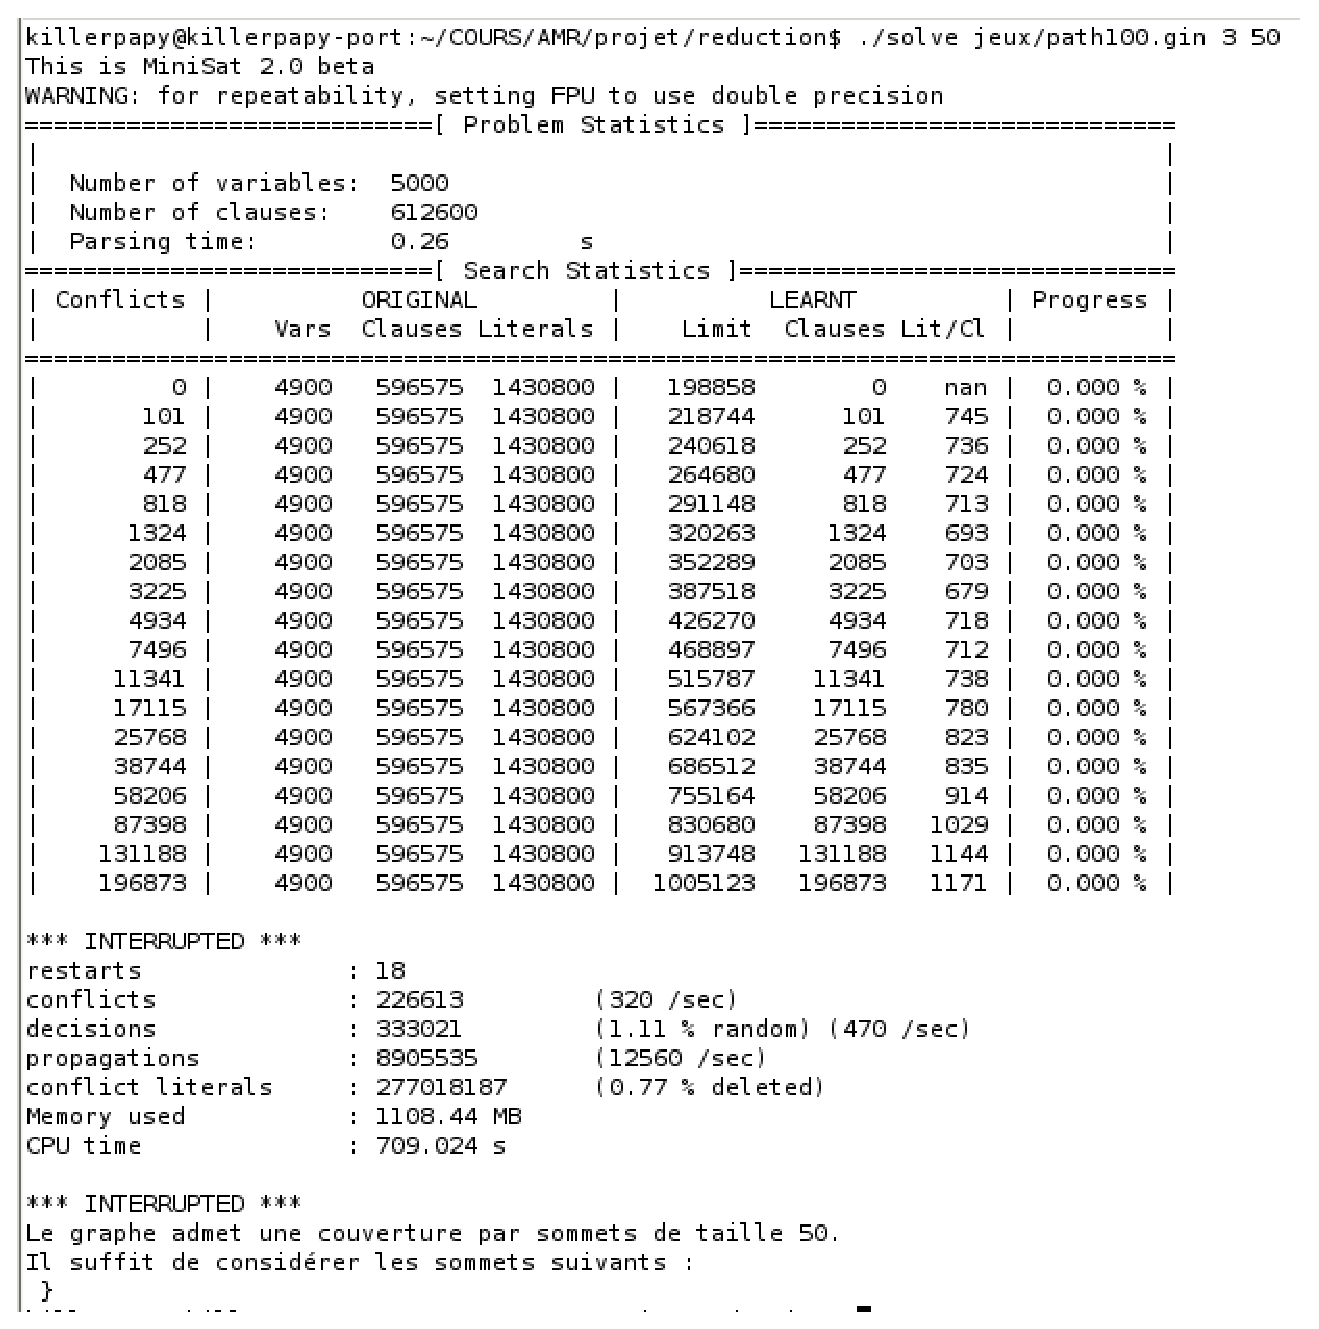
\includegraphics[width=12cm]{images/couv100.eps}
    \caption{\emph{Couverture par sommets} de taille 50 dans un path de
    taille 100.\label{lourd}}
   \end{center}
  \end{figure}

  \newpage

  \subsection{Annexe 2 \label{an2}}
  \emph{3-Kol} sur graphe \ref{graphe} page \pageref{graphe} de petite taille.
  \begin{figure}[!ht]
   \begin{center}
    \includegraphics[width=3cm,height=4cm]{images/jeurap.ps}
    \caption{Exemple de graphe à 4 sommets.\label{graphe}}
   \end{center}
  \end{figure}
  
  \begin{figure}[!ht]
   \begin{center}
    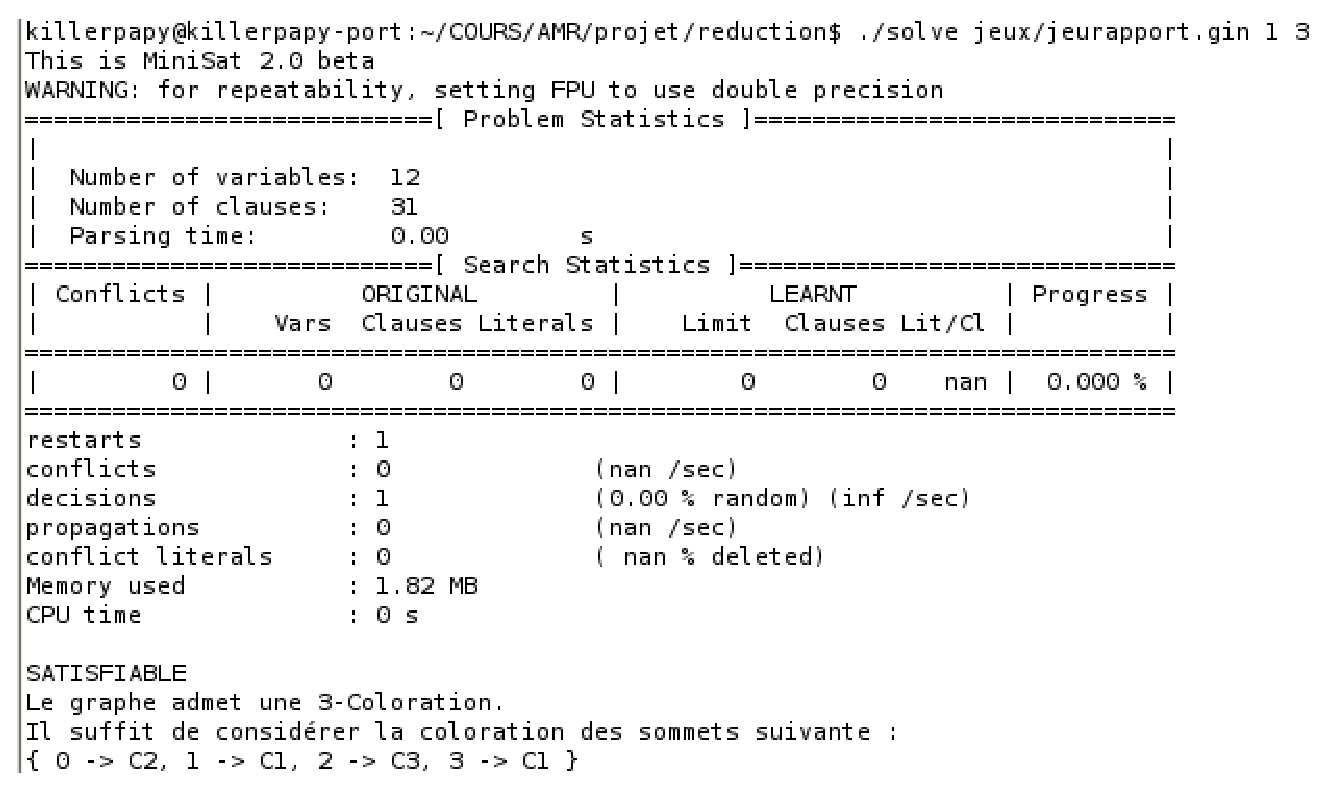
\includegraphics[width=12cm]{images/3-Kol.eps}
    \caption{Test de 3-Kol sur le graphe \ref{graphe}}
   \end{center}
  \end{figure}
  
  Ce qui donne comme résultat pour \emph{3-Kol}: \ref{result} page \pageref{result}
  \begin{figure}[!ht]
   \begin{center}
    \includegraphics[width=4cm,height=5cm]{images/jeurapport.ps}
    \caption{Test de 3-Kol sur le graphe \ref{graphe} \label{result}}
   \end{center}
  \end{figure}